\documentclass [a4paper, 12x `pt]{article}
\usepackage [utf8] {inputenc}
\usepackage [T2A] {fontenc}
\usepackage [russian] {babel}
\usepackage {amsmath, amsfonts, amssymb, amsthm}
\usepackage{graphicx}

\author{Александров Олег}

\begin{document}

\begin{titlepage}
   \begin{center}
        \hfill \break
        \footnotesize{ФЕДЕРАЛЬНОЕ ГОСУДАРСТВЕННОЕ БЮДЖЕТНОЕ ОБРАЗОВАТЕЛЬНОЕ УЧРЕЖДЕНИЕ}\\ 
        \footnotesize{ВЫСШЕГО ПРОФЕССИОНАЛЬНОГО ОБРАЗОВАНИЯ}\\
        \small{\textbf{«МОСКОВСКИЙ ФИЗКУЛЬТУРНЫЙ ТЕХНИКУМ С УГЛУБЛЕННЫМ ИЗУЧЕНИЕМ ИННОСТРАННЫХ ЯЗЫКОВ»} }\\
        \hfill \break
        \hfill \break
        \hfill \break
        \normalsize{«Физкек-школа прикольных мемов и инфоцыганства»}\\
        \hfill \break
        \hfill \break
        \hfill \break
        \normalsize{Кафедра? Я её не выбрал ещё...}\\
        \hfill\break
        \hfill \break
        \hfill \break
        \hfill \break
        \LARGE{«Начало математического безумия!!!»}\\
        \hfill \break
        \hfill \break
        \hfill \break
        \hfill \break
        \hfill \break
        \hfill \break
        \hfill \break
        \hfill \break
        \hfill \break
        \hfill \break
        \begin{center}
            \normalsize{Работу выполнил}
        \end{center}
        \begin{center}
            \normalsize{Александров Олег Алексеевич}
        \end{center}
        \hfill \break
        \normalsize{Долгопрудный 2023} 
    \end{center}
    \thispagestyle{empty}
\end{titlepage}

Дано f(x) = $$ \sin(x)  $$\\
Методом пристального взгляда заметим, что!
$$ \sin(x)  $$\\
\begin{figure}[h]
	\centering
	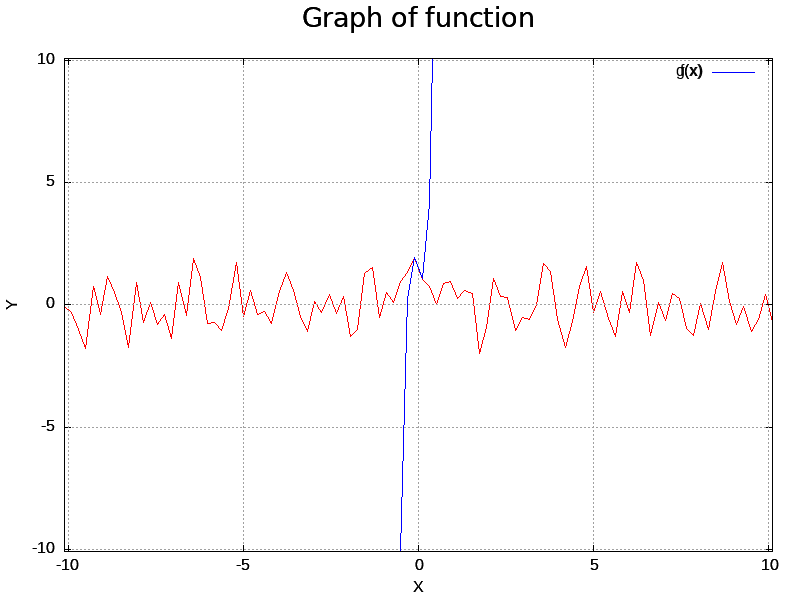
\includegraphics[width=0.8\linewidth]{Images/graphic0.png}
	\caption{\label xGraph of function.}
\end{figure}
"ДИРИХЛЕЕЕЕ!!! ДИРИХЛЕЕЕ!!!" - Савватеев А.В.
$$ \frac{d}{dx}(x) = 1 $$\\
Наносим 10 Сталинских ударов по этому выражению!!!
$$ \frac{d}{dx}(\sin(x) ) = \cos(x)  \cdot 1 $$\\
Вспоминаем метод Алекса Эдуардовича Султанова!!!
$$ \cos(x)  $$\\
В итоге производная f'(x) = $$ \cos(x)  $$\\
\begin{figure}[h]
	\centering
	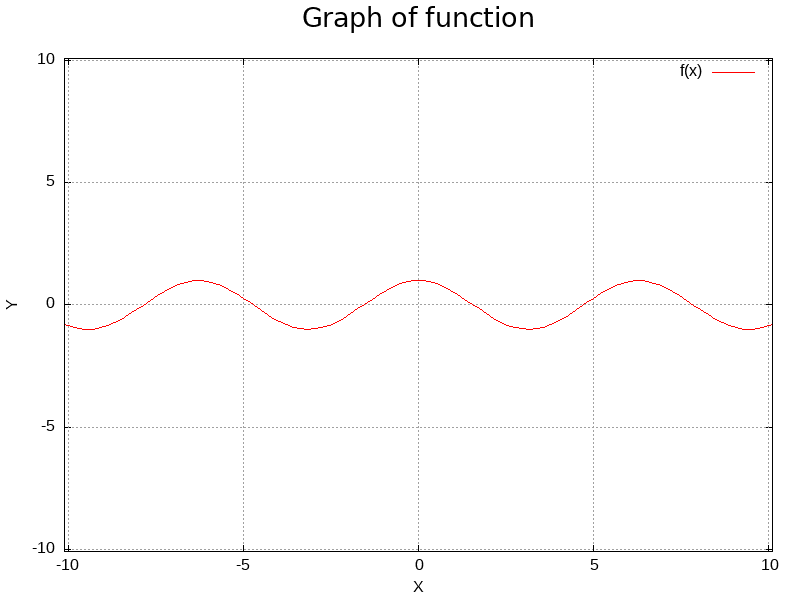
\includegraphics[width=0.8\linewidth]{Images/graphic1.png}
	\caption{\label xGraph of function.}
\end{figure}
Что это такое? А! Так это очевидно!!!
$$ \frac{d}{dx}(x) = 1 $$\\
Получим вот такое выражение! Мы упустили часть доказательств равносильных переходов! Поэтому я хочу, чтобы ВЫ САМИ ИХ ДОКАЗАЛИ!
$$ \frac{d}{dx}(\sin(x) ) = \cos(x)  \cdot 1 $$\\
Заметим, что ...
$$ \cos(x)  $$\\
Сейчас наступит катарсис!!!
$$ x $$\\
Наносим 10 Сталинских ударов по этому выражению!!!
$$ \frac{d}{dx}(x) = 1 $$\\
Вас ещё не кокнуло? Продолжаем!
$$ \frac{d}{dx}(\cos(x) ) = -1 \cdot \sin(x)  \cdot 1 $$\\
Заметим, что ...
$$ -1 \cdot \sin(x)  $$\\
Для решения этой задачи переместимся в n-мерное пр-во!!!
$$ x $$\\
Доказательство тривиально!!! Оставим читателю в качестве домашнего упражнения!
$$ \frac{d}{dx}(x) = 1 $$\\
Для решения этой задачи переместимся в n-мерное пр-во!!!
$$ \frac{d}{dx}(\sin(x) ) = \cos(x)  \cdot 1 $$\\
Вспоминаем метод Алекса Эдуардовича Султанова!!!
$$ \frac{d}{dx}(-1) = 0 $$\\
"ДИРИХЛЕЕЕЕ!!! ДИРИХЛЕЕЕ!!!" - Савватеев А.В.
$$ \frac{d}{dx}(-1 \cdot \sin(x) ) = 0 \cdot \sin(x)  + -1 \cdot \cos(x)  \cdot 1 $$\\
Сейчас наступит катарсис!!!
$$ -1 \cdot \cos(x)  $$\\
Доказательство тривиально!!! Оставим читателю в качестве домашнего упражнения!
$$ -0.166667 \cdot x^{3}  + x $$\\
Разложение в ряд Тейлора g(x) = $$ -0.166667 \cdot x^{3}  + x $$\\
\begin{figure}[h]
	\centering
	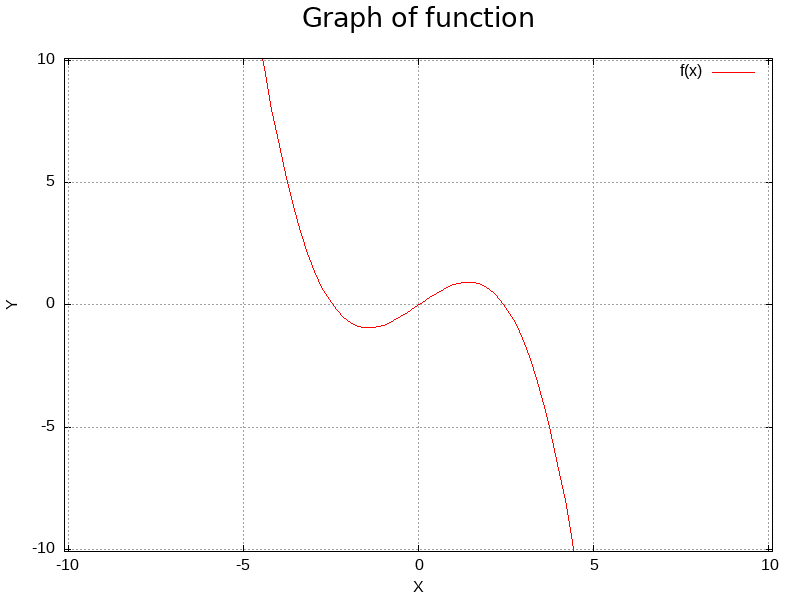
\includegraphics[width=0.8\linewidth]{Images/graphic2.png}
	\caption{\label xGraph of function.}
\end{figure}
Исходная функция: $$ \sin(x)  $$\\
Производная выражения: $$ \cos(x)  $$\\
Разложение в ряд Тейлора g(x) = $$ -0.166667 \cdot x^{3}  + x $$\\

\addcontentsline{toc}{chapter}{bibname}
\bibliographystyle{utf8gost705u}
\bibliography{biblio}

\end{document}
